\documentclass[sigconf]{acmart}

\usepackage{graphicx}
\usepackage{hyperref}
\usepackage{todonotes}

\usepackage{endfloat}
\renewcommand{\efloatseparator}{\mbox{}} % no new page between figures

\usepackage{booktabs} % For formal tables

\settopmatter{printacmref=false} % Removes citation information below abstract
\renewcommand\footnotetextcopyrightpermission[1]{} % removes footnote with conference information in first column
\pagestyle{plain} % removes running headers

\newcommand{\TODO}[1]{\todo[inline]{#1}}

\begin{document}

\title{Big Data Applications and Manufacturing}

\author{Borga Edionse Usifo}
\affiliation{%
\institution{Indiana University}
\city{Bloomington} 
\state{Indiana} 
\postcode{47408}
}
\email{busifo@iu.edu}

\renewcommand{\shortauthors}{B. Usifo et al.}

\begin{abstract}
Technology is starting to change the way of industrial operations since the competitiveness is getting more prominent for companies their quality metrics and tolerances are getting smaller every day to make the quality items. We will explain the importance of essential data applications in manufacturing operations. These operations are consist of supply chain associated with manufacturing, intelligence systems in manufacturing, leverage of Big Data applications, as well as intelligence systems in factory processes.
\end{abstract}

\keywords{i523, HID343, Manufacturing, Industry 4.0, Autonomous Decision in Manufacturing, Analytics in Manufacturing}

\maketitle
%%%%%%%%%%%%%%%%%%%%%%%%%%%%%%%%%%%%%%%%%%%%%%%%%%%%%%%%%%%%%%%%%%%%%%%%%%%%%%%%%%%%%%%%%%%%%%%%%%%%%%%%%%%%%%%%%%%%%%%%%%%%%%%%%%%%%%%%%%%%%%%%%%%%%%%%%

\section{Introduction}

It was a big step forward when Henry Ford introduced first moving assembly line production in manufacturing processes \cite{www-ford}. This innovative approach drastically improved the efficiency of the assembly time of making a car from start to finish \cite{www-history}. Previous to Henry Ford's invention, assembly of the similar car could take up to twelve hours after the invention this time reduced to only thirty minutes \cite{www-history}. This invention brought another aspect to the world of manufacturing which was the reducing the waste of manufacturing operations to make faster and efficient process to supply demand \cite{www-industryweek}.

\par Since from Henry Ford's invention, manufacturing is transforming, and it is updating itself with technological advancements for modernized operations. 

%%%%%%%%%%%%%%%%%%%%%%%%%%%%%%%%%%%%%%%%%%%%%%%%%%%%%%%%%%%%%%%%%%%%%%%%%%%%%%%%%%%%%%%%%%%%%%%%%%%%%%%%%%%%%%%%%%%%%%%%%%%%%%%%%%%%%%%%%%%%%%%%%%%%%%%%%

\section{Importance of Data-Driven Approach in Manufacturing}

Improvements in machine connectivity to computer networks, in other words, Internet of Things (IoT), made possible to extract actionable data from automated processes this approach defines as data-driven decision in manufacturing processes \cite{data-driven, HE2017}.

\par We can divide this importance into four categories which are crucial for any lean operation in manufacturing \cite{www-leanblog}. These categories are quality, cost, delivery, and most importantly safety \cite{www-leanblog}.


\subsection{Quality}

Industry approach of inspecting the defective item transformed with the modern approach of having a statistical quality controlled processes to prevent or catch defectiveness before happening. This approach goes back to Bells Laboratories when Dr. Walter Schewart introduced to statistical quality control to prevent defects \cite{yusof1998}.

\par Demand for quality products is massively increasing. This increase also putting pressure on companies to make more bespoke products with lower manufacturing tolerances \cite{OLIFF2017167}. This demand and complex operations shifting industry to seek or develop intelligence systems to supply bespoke customer demand \cite{OLIFF2017167}.``Estimates by government agencies put the potential gains in efficiency of such processes as high as 30\% \cite{OLIFF2017167}.`` 

\subsection{Cost}
Manufacturing cost can put into three subcategories these categories are \cite{www-wikipedia};

\begin{itemize}
    \item Direct material cost
    \item Direct labor cost
    \item Manufacturing overhead
\end{itemize}

Organizations need to adopt changes quickly and efficiently for staying, and even improving their competitiveness in their business areas \cite{HAMMER2017715}. Data-driven decision enables organizations to find the best process model for their optimal operating costs \cite{HAMMER2017715}.``Advanced analytics help capture the full impact by incorporating trade-offs such as yield, throughput, energy and raw material consumption in one single profitability metric \cite{HAMMER2017715}.``

\subsection{Delivery}
As we stated before most crucial philosophy in manufacturing sector is eliminating waste \cite{www-toyota}. Moreover, having produced more than needed puts companies under pressure of losing critical inventory capabilities. Toyota Production System(TPS) which has a philosophy of ``the complete elimination of all waste`` brought another philosophy on delivery capabilities \cite{www-toyota}. This philosophical approach is called Just-In-Time(JIT) which means ``only what is needed, when it is needed, in the amount needed \cite{www-toyota}``.

Growing real-time data from digital machines, cell phones, GPS signals, and other intelligent systems flooding into the global logistics industry and it is forcing the industry to gain competitive leverage from this data to adjust their demand and capacity fluctuations \cite{ZHONG2016572}. This data-driven approach opens new doors on not just having a JIT system implemented but also gives a predictive approach to customer demand. 

%%%%%%%%%%%%%%%%%%%%%%%%%%%%%%%%%%%%%%%%%%%%%%%%%%%%%%%%%%%%%%%%%%%%%%%%%%%%%%%%%%%%%%%%%%%%%%%%%%%%%%%%%%%%%%%%%%%%%%%%%%%%%%%%%%%%%%%%%%%%%%%%%%%%%%%%%

\section{How it related to big data analytics for the manufacturing}

There are many application areas of Big Data technologies and research related to Big Data \cite{BABICEANU2016128}. Manufacturing applications are insufficient when compared to information science, healthcare, and other business processes \cite{BABICEANU2016128}. Most important of Big Data research is data analysis without analytical approach other aspects of Big Data which are the collection, storage, and use will not add too much value to Big Data research \cite{BABICEANU2016128}. 

\par There are requirement tools and techniques for processing of Big Data. These resources include ``process capability, memory, storage, and networks, such as Hadoop Distributed File System (HDFS), MapReduce, YARN, HBase, HiveQL, NoSQL, and other \cite{BABICEANU2016128}.``

\par Standardization required for Big Data applications, which we can refer to these standardization as dimensions of Big Data applications. Three most fundamental dimensions are \cite{BABICEANU2016128, ZHONG2016572}:

\begin{itemize}
    \item Volume: Data is no longer in small amounts its made by a significant amount. ``It is calculated that a personal care manufacturer generates 5000 data samples every 33ms, resulting in 152,000 samples per second, 9 million per minute, 13 billion per day, and 4 trillion samples per year.``
    \item Variety: There are diverse data formats due to it is heterogeneous nature. 
    \item Velocity: Data needs to flow/generate continuously, and velocity relies on speed of data collection
\end{itemize}

\par There are several attempts for assigning more dimensions to Big Data due it is enlarging characteristics. These additional dimensions are as follows \cite{BABICEANU2016128}: 

\begin{itemize}
    \item Value: Each work, each motion, and each data needs to add value to any information gain
    \item Veracity: Data needs to protected from outside influences and needs to be statistically reliable to make decision
    \item Vision: Data should come from a purposeful process
    \item Verification: Engineering measurements and data should correlate with each other
    \item Variability: Variation in the data which addresses the inconsistency and approximation. 
    \item Volatility: Old data should easily replaceable with a new generated data source because old data may have expiration cycle.
    \end{itemize}
    
\par Process flows as shown in Figure for accurate Big Data implementation Figure \ref{fig:5V}.  

 \begin{figure}[!ht]
  \centering
      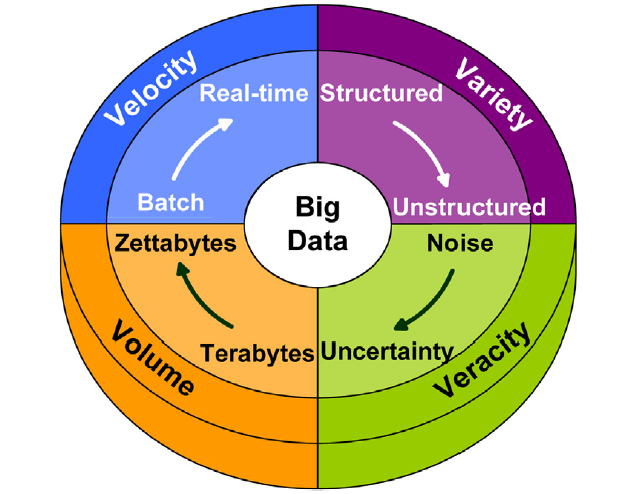
\includegraphics[width=\columnwidth]{images/5V.png}
  \caption{Process Flow of V's for accurate data gathering \cite{HE2017}.}\label{fig:5V}
\end{figure}
    
\par This additional dimensions improves the quality and characteristics of data, which collected from manufacturing processes and any related applications \cite{BABICEANU2016128}.
\par Some reports have been shown that Big Data analytics is enabling manufacturing operations to get timely and accurate insights from data to continuously improve for better manufacturing operations while using ``predictive analysis, machine learning, HUFFS, and Map Reduce tools \cite{BABICEANU2016128}.``  

%%%%%%%%%%%%%%%%%%%%%%%%%%%%%%%%%%%%%%%%%%%%%%%%%%%%%%%%%%%%%%%%%%%%%%%%%%%%%%%%%%%%%%%%%%%%%%%%%%%%%%%%%%%%%%%%%%%%%%%%%%%%%%%%%%%%%%%%%%%%%%%%%%%%%%%%%

\section{Analytics Used on Manufacturing Operations}

 Every day smart factories are emerging and improving themselves with the help of technological advances this smart factory revolution called as Industry 4.0 which ``formed in by National Academy of Science and Engineering and it is working group founded on the Hanover exhibition in the year 2011 \cite{WAGNER2017125}.`` 

\par Definition of Industry 4.0 is the technical perspective ``people and things to be connected Anytime, Anyplace, with Anything and Anyone, ideally using Any path/network and Any service \cite{saint-exupery}``. Fundamental technologies for Industry 4.0 are cyber-physical systems(CPS) and applications on CPS in manufacturing are called cyber-physical production system (CPPS) \cite{WAGNER2017125}. This application made ``possible for data processing, machine to machine communication and human-machine interaction \cite{WAGNER2017125}``. We can categorize these CPPS elements into three main subjects:

\begin{itemize}
    \item Data acquisition and data processing
    \item Machine to machine communications (M2M)
    \item Human-machine interaction (HMI) \cite{WAGNER2017125}.
\end{itemize}

\par There are several areas that Big Data has been gaining size in manufacturing operation. Industry 4.0 applications mostly focused areas are:

\begin{itemize}
    \item Predictive maintenance \cite{KUMAR2017}
    \item Big Data Analytics in Supply Chain  \cite{WANG201698}
    \item Statistical process monitoring for smart manufacturing \cite{HE2017} 
\end{itemize}


\subsection{Predictive Maintenance with Big Data Analytics}
Economic loses of unexpected maintenance on manufacturing operations can have a devastating effect and can significantly increase waste. Furthermore, unexpected events can also put the Just-In-Time system design into jeopardy which will also have a significant effect on the customer to not having the ordered item on time. Predictive-based maintenance approach can minimize this kind of economic losses and can improve the customer service \cite{KUMAR2017}.Preventative maintenance consists of five parts: `` data collection and acquisition, data pre-processing, failure detection, failure isolation and failure identification \cite{KUMAR2017}.``

\par To achieve optimal decision for successful predictive maintenance, connection and information gathering between different machinery, monitoring of individual equipment health, and self-adapting modeling have to come in to play together \cite{HE2017}. 

\subsection{Statistical Process Monitoring for Smart Manufacturing}

As we stated before the first version of statistical process monitoring (SPM) was found in Bell Laboratories which was successfully reduced the additional adjustments as well as improved the production quality inside process by analyzing statistical distribution method of normal distribution. It was estimating the mean ($\overline{m}$) and the standard deviation $\sigma $. Anything outside the ($\overline{m}\pm 3\sigma$) is considered to take an action point or investigation point for assignable cause \cite{HE2017}. The major drawback for SPM was to fail to detect two properties of an item whenever the fault occurs.


\par Second versions of statistical process control introduced in 1980's which called multivariate statistical process monitoring (MSPM). The underlying statistical method was ``exploring correlations between process and quality variables \cite{HE2017}``. This method was more robust when identifying the fault when two or more properties were in action and as a result, they widely used in manufacturing processes \cite{HE2017}. There are also some limitations with the MSPM when there is ``non-linear relationship between variables, present outliers, failed sensors, multimodal distribution \cite{HE2017}.``



\par Third version of statistical controls are still emerging, and this is the part where new Big Data analytical techniques come into play. These analytical techniques expected to utilize more information which lacks on the first and second generation and expected to become an essential basis of profitability, quality, and many more aspects.

\subsection{Big Data Analytics in Supply Chain }

Big Data applications have been gaining more place in supply chain analytics (SCA). Some these applications are `` demand planning, procurement, production, inventory, and logistics \cite{WANG201698}``. 

\subsubsection{Procurement}

SCA gives distinguishable insights about trends in markets and gives monitoring abilities to adjust their organizational needs. These analytical approaches can also help avoid any future risks from organizations. Another power of SCA is monitoring suppliers performances based on their sourcing abilities \cite{WANG201698}. 

\subsubsection{Production}

Supply chain analytics will let manufacturing operations to analyze and understand production cost and their influence in each manufacturing processes capacities. This will let management to take quick actions on improvement if any needed \cite{WANG201698}.

\subsubsection{Inventory}
Inventory levels are one of the highest priority in any manufacturing operations because it correlated with waste in the operations \cite{www-toyota}. SCA can help predict inventory levels more accurately such as demand from the customer and adjusting supply for demand \cite{WANG201698}. 

\par We just investigate the areas of the supply chain that affected by the recent improvements in Big Data and Analytics. Analytics that used in these applications are 

\par Widely used traditional supply chain analytics are ``time series analysis and forecasting and regression analysis`` because of data generated from organizations are getting larger these traditional techniques becoming less effective. There are new complex algorithms needed to analyze massive data \cite{WANG201698}. 

\par Traditional optimization techniques are also slow, and they are not accurate if there is a significant amount of data. To improve the accuracy of optimization techniques it is essential to support optimization's with `` parallel computing, randomized and approximation algorithms, and simplify implementations \cite{WANG201698}.``







%%%%%%%%%%%%%%%%%%%%%%%%%%%%%%%%%%%%%%%%%%%%%%%%%%%%%%%%%%%%%%%%%%%%%%%%%%%%%%%%%%%%%%%%%%%%%%%%%%%%%%%%%%%%%%%%%%%%%%%%%%%%%%%%%%%%%%%%%%%%%%%%%%%%%%%%%

\section{Conclusion}

We presented the importance of smart manufacturing and Big Data based applications on Industry 4.0 (smart manufacturing). Insights about advantages of predictive maintenance, statistical control techniques, smart supply chain innovations had given. Several analytical approaches while using Big Data applications also had shown.

\begin{acks}

The author would like to thank Dr. Gregor von Laszewski for his support and suggestions to write this paper.

\end{acks}

\bibliographystyle{ACM-Reference-Format}
\bibliography{report} 



\end{document}
